\documentclass[a4paper,11pt]{article}
%@@@@@@@@@@@@@@@@@@@@@@@@@@@@@@@@@@@@@@@@@@@@@@@@@@@@@@@@@@@
%@@@@@@@@@@@@@@@@      PACOTES BÁSICOS		     @@@@@@@@@@
%@@@@@@@@@@@@@@@@@@@@@@@@@@@@@@@@@@@@@@@@@@@@@@@@@@@@@@@@@@@

\usepackage[T1]{fontenc}
\usepackage[utf8]{inputenc}
\usepackage{lmodern} 
\usepackage[portuguese]{babel}
\usepackage{amsmath}
\usepackage{array}
\usepackage{graphicx}				%para imagens
\usepackage{epstopdf} 				%resolve problemas eps-pdf
\usepackage{pict2e}				%%writting to images
%@@@@@@@@@@@@@@@@@@@@@@@@@@@@@@@@@@@@@@@@@@@@@@@@@@@@@@@@@@@
%@@@@@@@@@@@@@@@@     PACOTES NÃO TAOBÁSICOS		 @@@@@@@@@@
%@@@@@@@@@@@@@@@@@@@@@@@@@@@@@@@@@@@@@@@@@@@@@@@@@@@@@@@@@@@
\usepackage{fancyhdr}				% para o cabeçalho bonito
\usepackage{caption}					%para legendas
\usepackage{subcaption}				% e sublegendas
\usepackage{placeins} 				%controlar o lugar dos floats
\pagestyle{fancy} 					% número de pag e cabeçalho
\usepackage{txfonts} 				%fontes bonitas? acho que para o título
\usepackage[usenames]{color} 		% algo com gunplot e eps
\usepackage{ifthen}
\usepackage{xparse}
\graphicspath{{./../images/}{./../data/}{./graph/}}	% procura imagens nessa pasta
\usepackage{float} %%para definir ambiente gráfico
\newfloat{Gráfico}{hbtp}{lop}[section]
%\usepackage{undertilde}	%%para notação de vetor do yuri
\usepackage[import]{xy} % para escrever em imagens
\xyoption{import}

\usepackage{listings}
\lstset{frame=single,}
%@@@@@@@@@@@@@@@@@@@@@@@@@@@@@@@@@@@@@@@@@@@@@@@@@@@@@@@@@@@
%@@@@@@@@@@@@@@@@      Cabeçalho de cada página      @@@@@@@
%@@@@@@@@@@@@@@@@@@@@@@@@@@@@@@@@@@@@@@@@@@@@@@@@@@@@@@@@@@@
\setlength{\headheight}{25pt}%compila sem erro
	\fancyhead{}
	\fancyfoot{}
	\fancyhead[R]{Sistemas de Medição}%direito superior
	\fancyhead[L]{
\includegraphics[height=0.25in]{./../images/logo_unb.pdf}}%esquerda superior
	\fancyfoot[C]{\thepage}%baixo centro
%E: Even page, O: Odd page, L: Left field, C: Center field, R: Right field, H: Header, F: Footer
% em documentos com dois lados use LO, RO. como esse documento não tem lados essa opção é inútil


%@@@@@@@@@@@@@@@@@@@@@@@@@@@@@@@@@@@@@@@@@@@@@@@@@@@@@@@@@@@
%@@@@@@@@@@@@@@@@      NOVOS COMANDOS		      @@@@@@@@@
%@@@@@@@@@@@@@@@@@@@@@@@@@@@@@@@@@@@@@@@@@@@@@@@@@@@@@@@@@@@
\newcommand\undermat[2]
	{
	  \makebox[0pt][l]
	  	{$\smash{\underbrace{\phantom{%
    \begin{matrix}#2\end{matrix}}}_{\text{$#1$}}}$
    		}#2
    	}
    	
\newcommand{\HRule}
	{
	\rule{\linewidth}{0.5mm}
	}
	
\newcommand{\EmptyPage}
	{
	\thispagestyle{empty}
	\mbox{ }
	\newpage	
	} 
	
\newcommand{\MakeMyTitlePage}[4]
%%Argumentos: 
%1º Nome da Matéria
%2º subtítulo ex: experimento IV
%3º título
%4º autores
% exemplo de autores:
%	\begin{center} \large
%		\begin{tabular}{llr} \
%		& & \\[0.05cm]		
%		Professora & Nadia Maria de Liz Koche & \\
%		
%		Alunos:& & \\
%		& Juarez A.S.F 					& 11/0032829\\
%		& Sérgio Fernandes da Silva Reis & 11/0140257\\
%		& Jedhai Pimentel				& 09/0007883\\	[0.05cm]	
%		\end{tabular}
%	\end{center}
{
\begin{titlepage}
\begin{center}

% Upper part of the page. The '~' is needed because \\
% only works if a paragraph has started.

\includegraphics[width=\textwidth]{./../images/logo_unb.pdf}~\\[1cm]

\Huge #1\\[0.5cm]

\huge #2

% Title
\HRule \\[0.4cm]
{ \huge \bfseries  #3}\\[0.4cm]

\HRule \\[0.5cm]

{\large \today}


\vfill %%o que vier depois vai ao fim da páginda


%Autor e Professor
\begin{center} \large
#4
\end{center}

\end{center}
\end{titlepage}

\EmptyPage
\tableofcontents
\newpage

}
	
%@@@@@@@@@@@@@@@@@@@@@@@@@@@@@@@@@@@@@@@@@@@@@@@@@@@@@@@@@@@
%@@@@@@@@@@@@@@@@      NOVOS AMBIENTES		      @@@@@@@@@
%@@@@@@@@@@@@@@@@@@@@@@@@@@@@@@@@@@@@@@@@@@@@@@@@@@@@@@@@@@@
\newcounter{graph-c}
\setcounter{graph-c}{0}


%\NewDocumentEnvironment{Graph}{m}
 % {%antes
  %\addtocounter{graph-c}{1}
  %\begin{figure}
  %}
 %{
 %depois
%	\end{figure} 
%	\caption*{Grafico \arabic{graph-c} - #1}
 %}

















%inclui todosos pacotes utilizados

\newcommand{\MyBox}[1]
{
	\begin{tabular}{|l|}\hline
	  #1 \\ \hline	    
	\end{tabular} 	
}

\lstset{frame=single,}	

\begin{document}



\MakeMyTitlePage
{Análise Dinâmica Linear}
{Experimento II}
{Simulink}
{%autores
		\begin{tabular}{llr} \
		& & \\[0.05cm]		
		Professor & Henrique Cezar Ferreira & \\
		
		Alunos:& & \\
		& Juarez A.S.F 					& 11/0032829\\
	[0.05cm]	
		\end{tabular}
}

%@@@@@@@@@@@@@@@@@@@@@@@@@@@@@@@@@@@@@@@@@@@@@@@@@@@@@@@@@@@
%@@@@@@@@@@@@@@@@      OBJETIVOS      @@@@@@@@@@@@@@@@@@@@@@
%@@@@@@@@@@@@@@@@@@@@@@@@@@@@@@@@@@@@@@@@@@@@@@@@@@@@@@@@@@@
\section{Objetivos}
\paragraph{}Utilizar o Simulink para analisar um sistema elétrico,
um dinâmico e um sistema genérico representado por diagrama de blocos.
%@@@@@@@@@@@@@@@@@@@@@@@@@@@@@@@@@@@@@@@@@@@@@@@@@@@@@@@@@@@
%@@@@@@@@@@@@@@        INTRODUÇÃO       @@@@@@@@@@@@@@@@@@@@ 
%@@@@@@@@@@@@@@@@@@@@@@@@@@@@@@@@@@@@@@@@@@@@@@@@@@@@@@@@@@@
\section{Introdução Teórica}
\paragraph{} No estudo de controle de sistemas dinâmicos é recorrente
utilizar a função de transferência de um sistema para prever sua resposta
a uma determinada entrada. Uma vez conhecida a função de transferência 
e a transformada de Laplace da entrada I(s) podemos determinar a saída
através da transformada inversa de Laplace. O cálculo da transformada 
inversa requer muitas vezes o uso de frações parciais ou ainda de uma 
integral de convolução. A utilização desses métodos nos dá a forma
analítica da saída, mas sem sempre isso é necessário. Muitas vezes
podemos usar ferramentas computacionais para conhecer graficamente 
a resposta do sistema. Uma ferramente que permite essa análise é
o Simulink.

\paragraph{}No Simulink o sistema pode ser representado na forma
de diagrama de blocos. Existem 2 blocos ou operações fundamentais
utilizados nessa representação: bloco de função de transferência e
bloco somador. A figura \ref{fig:circuit2} mostra um diagrama de blocos
que será usado mais tarde. Os retângulos com G's dentro são os blocos
função de transferência. O sinal que entra neles sai multiplicado pela 
função de transferência descrita em seu interior. O bloco somador é 
representado pelo círculo com uma cruz. O sinal de saída desse bloco 
é a soma ou diferença das suas entradas. A operação que esse bloco
realiza é indicado pelo sinal junto a suas entradas. Vale ainda notar
que o diagrama é orientado e o sentido do fluxo de sinal em uma conexão 
de blocos é indicado pela ponta da seta. 
 
 \paragraph{} Com essas simples operações podemos implementar em blocos
 o comportamento de diversas equações diferenciais. Utilizando as propriedades
 da transformada de Laplace podemos representar a derivação no domínio do tempo
 por uma multiplicação por s no domínio da frequência, ou ainda uma integração
 no tempo por uma multiplicação por $\frac{1}{s}$ na frequência. Podemos ainda
 representar um circuito inteiro pelo bloco com sua função de transferência.

\paragraph{} O interessante do uso de diagramas de blocos é poder
abstrair o sistema que ele representa. Isto é, podemos nos concentrar
no efeito que as relações entre os componentes causa sem nos preocuparmos
com os detalhes dos componentes em si. Dessa forma podemos usar as mesmas 
técnicas para analisar sistemas das mais diversas naturezas, depois
de obtidas as funções de transferência os sistemas físicos serão resolvidos
da mesma forma, seja ele elétrico, mecânico ou que for. 

\begin{figure}[!htp]
	\begin{subfigure}[!htp]{0.5\textwidth}
		\centering
		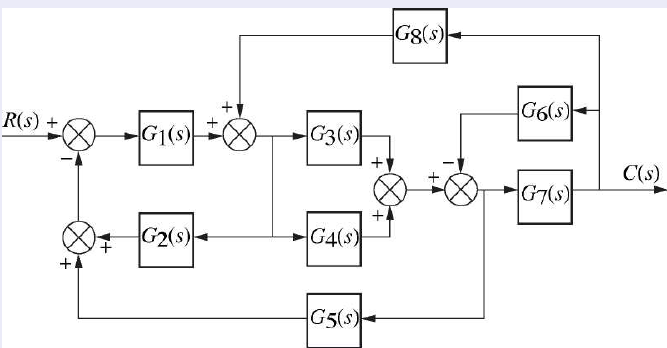
\includegraphics[scale = 0.5]{./images/exp2-exerc2.png}
		\caption{exemplo de diagrama de blocos}
		\label{fig:circuit2}
	\end{subfigure}		
	\caption{}
\end{figure}

%@@@@@@@@@@@@@@@@@@@@@@@@@@@@@@@@@@@@@@@@@@@@@@@@@@@@@@@@@@@
%@@@@@@@@@@@@       PROCEDIMENTOS        @@@@@@@@@@@@@@@@@@@
%@@@@@@@@@@@@@@@@@@@@@@@@@@@@@@@@@@@@@@@@@@@@@@@@@@@@@@@@@@@
\newpage
\section{Descrição Experimental}
	\subsection{Exercício 1}
\FloatBarrier
\begin{figure}[!htp]
	\begin{subfigure}[!htp]{0.5\textwidth}
		\centering
		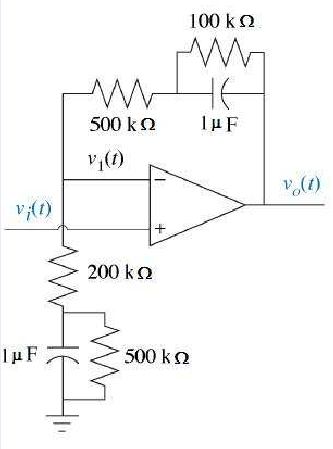
\includegraphics[scale = 0.5]{./images/exp2-circuit1.png}
		\caption{}
		\label{fig:circuit1}
	\end{subfigure}
	\begin{subfigure}[!htp]{0.5\textwidth}
		\centering
		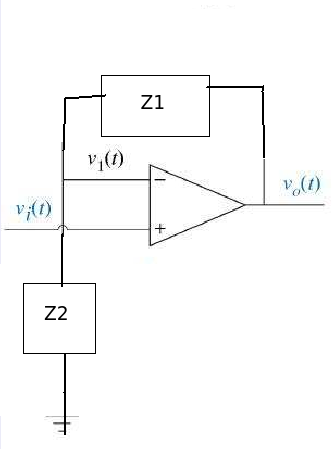
\includegraphics[scale = 0.5]{./images/exp2-circuit1-simplified.png}
		\caption{circuito generalizado}
		\label{fig:circuit1-simplified}
	\end{subfigure}
		
	\caption{Circuito do exercício 1}
\end{figure}
\FloatBarrier
\paragraph{}Considere o circuito na figura \ref{fig:circuit1}. 
Desejamos calcular a função de transferência H(s) que relaciona
a saída com a entrada. Para facilitar o desenvolvimento considere
o circuito genérico na figura \ref{fig:circuit1-simplified}. 
A função de transferência pode ser facilmente calculada a partir
do modelo ideal para o amp op que considera que seus terminais
+ e - estão em um curto circuito virtual e que a corrente por 
eles é nula. Nesse caso a função de transferência é:

\begin{equation}
	H(s) = \frac{Z_1 + Z_2}{Z_2}
	\label{eq:exerc1-H}
\end{equation}
\paragraph{}Substituindo os valores do problema podemos achar 
a saída para o caso em estudo. Para facilitar notamos que as 
resistências envolvidas são todas múltiplas de 100k$\Omega$
e podemos colocá-las em termos de R = 100k$\Omega$. O código
de matlab a seguir utiliza essa ideia para simplificar os 
cálculos. Ele calcula a função de transferência e a exibe 
na tela já em forma simplificada.

	\lstinputlisting{./../Matlab/exercicio1FindTF.m}

\paragraph{}Com a função de transferência obtida podemos 
montar o diagrama de blocos no Simulink e simular a resposta
do circuito a diversas entradas, em particular simularemos 
a saída ao degrau unitário. A montagem do diagrama de blocos 
é ilustrada a seguir. Vemos também a janela de configuração
do bloco de função de transferência onde especificamos 
o numerador e o denominador de H(s).
\FloatBarrier
\begin{figure}[!htp]
		\centering
		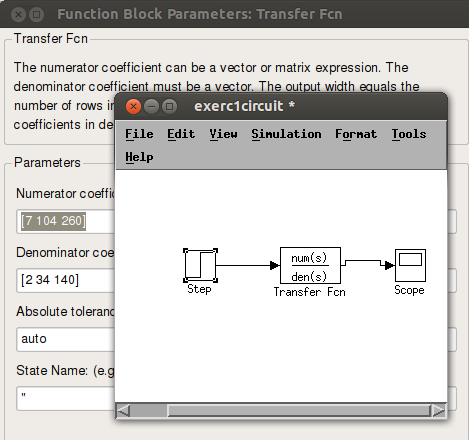
\includegraphics[scale = 0.5]{./images/circuit1-diagrama.png}
	\caption{diagrama de blocos da simulação no Simulink}
\end{figure}
\FloatBarrier
\subsection{Exercício 2}
\paragraph{}Agora montamos o diagrama de blocos como na figura
\ref{fig:exerc2-diagram} e simulamos a resposta ao degrau unitário.
\FloatBarrier
\begin{figure}[!htp]
		\centering
		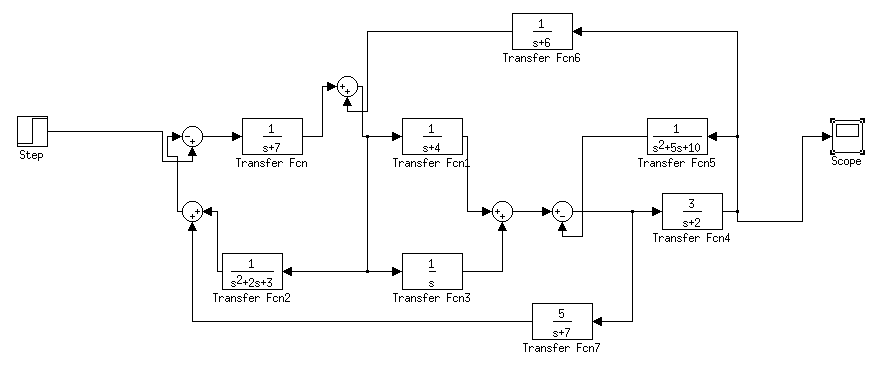
\includegraphics[scale = 0.6]{./images/exp2-circuit2-diagram.png}
	\caption{diagrama de blocos}
	\label{fig:exerc2-diagram}
\end{figure}
\FloatBarrier

\subsection{Exercício 3}
\paragraph{}Estudamos agora o sistema mecânico na figura
\ref{fig:exerc3-diagram} com os valores de todas as 
constantes envolvidas iguais a 1. A  figura \ref{fig:exerc3-matlab}
mostra o diagrama da montagem no Simulink junto com a configuração 
do sinal de entrada. Em uma segunda parte tentamos simular a resposta
a um impulso ao reduzir o tamanho de pulso para 0.05s e subir a amplitude
para 100V. Usamos também a função impulse para comparar os resultados.

\FloatBarrier
\begin{figure}[!htp]
		\centering
		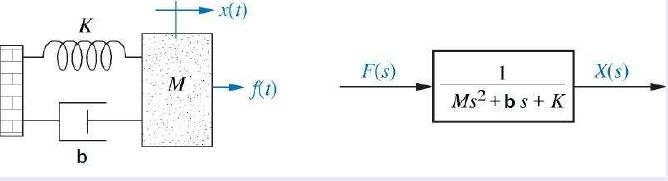
\includegraphics[scale = 0.6]{./images/exp2-problem3.jpg}
	\caption{sistema mecânico e sua função de transferência}
	\label{fig:exerc3-diagram}
\end{figure}
\begin{figure}[!htp]
		\centering
		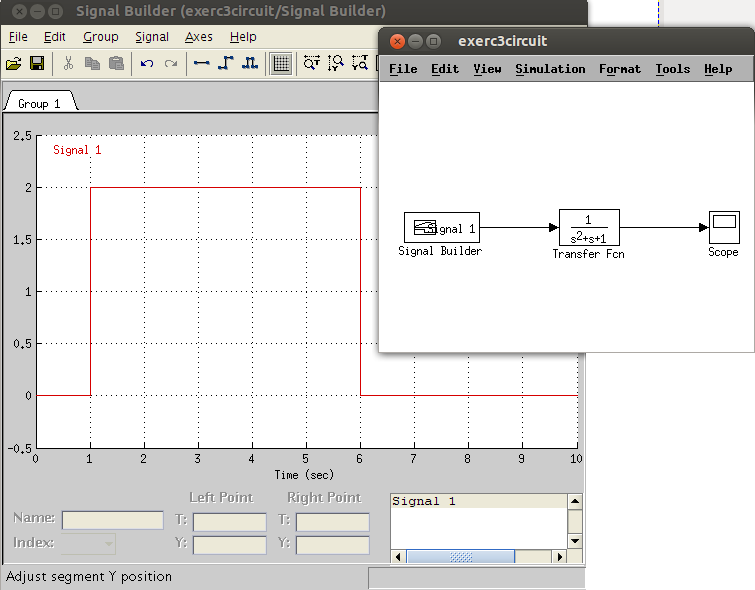
\includegraphics[scale = 0.6]{./images/exp2-circuit3-montagem.png}
	\caption{}
	\label{fig:exerc3-matlab}
\end{figure}

\FloatBarrier
%@@@@@@@@@@@@@@@@@@@@@@@@@@@@@@@@@@@@@@@@@@@@@@@@@@@@@@@@@@@
%@@@@@@@@@@@@@@@@@@@       DADOS      @@@@@@@@@@@@@@@@@@@@@@
%@@@@@@@@@@@@@@@@@@@@@@@@@@@@@@@@@@@@@@@@@@@@@@@@@@@@@@@@@@@
 \newpage
\section{Resultados}

	\subsection{Exercício 1}
		\paragraph{} A saída da rotina para cálculo da função 
é apresentada a seguir:
	\begin{lstlisting}[frame=single]
     2
  7 s  + 104 s + 260
  ------------------
     2
  2 s  + 34 s + 140
	\end{lstlisting}
A função de transferência é salva na variável H e podemos usar
o comando latex(H) para obter o código e apresentar a resposta
adequadamente em formato texto:
\begin{equation}
\frac{7\, s^2 + 104\, s + 260}{2\, s^2 + 34\, s + 140}
\end{equation}
A saída da simulação de resposta ao degrau unitário é 
apresentada a seguir:
\begin{figure}[!htp]
		\centering
		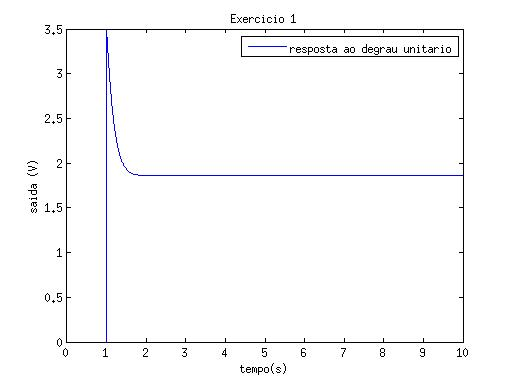
\includegraphics[scale = 0.5]{./images/exerc1-saida.jpg}
		\caption{resposta ao impulso unitário}
		\label{fig:circuit1}
\end{figure}

\subsection{Exercício 2}
\paragraph{}A resposta ao degrau unitário é mostrada no gráfico a seguir:
\FloatBarrier
\begin{figure}[!htp]
		\centering
		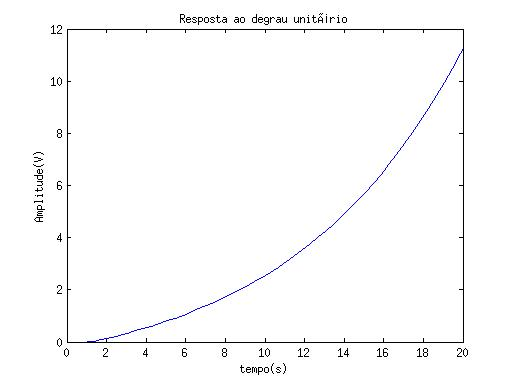
\includegraphics[scale = 0.5]{./images/exerc2-saida.jpg}
		\caption{resposta ao impulso unitário}
		\label{fig:circuit2-saida}
\end{figure}
\FloatBarrier
vemos que a saída apresenta comportamento exponencial.

\subsection{Exercício 3}
\paragraph{}A resposta obtida é mostrada no gráfico \ref{fig:circuit3-saida}.
A reposta obtida a simulação de um impulso por um pulso de amplitude 100V e duração
0.05s é mostrada na figura \ref{fig:circuit3-impulso-simulado} e a saída da função impulse
na figura \ref{fig:circuit3-impulso-pro}.
\FloatBarrier
\begin{figure}[!htp]
		\centering
		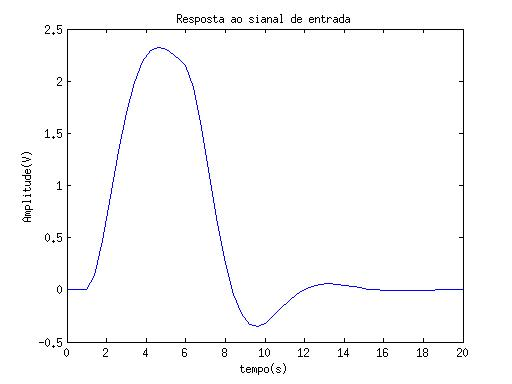
\includegraphics[scale = 0.5]{./images/exerc3-saida.jpg}
		\caption{resposta do sistema mecânico}
		\label{fig:circuit3-saida}
\end{figure}
\begin{figure}[!htp]
		\centering
		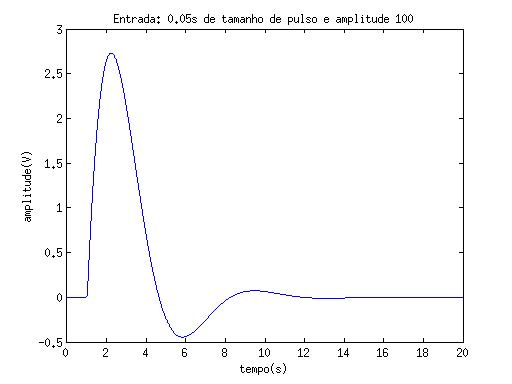
\includegraphics[scale = 0.5]{./images/exerc3-saida-impulso-simulado.jpg}
		\caption{resposta com aproximação de impulso}
		\label{fig:circuit3-impulso-simulado}
\end{figure}
\begin{figure}[!htp]
		\centering
		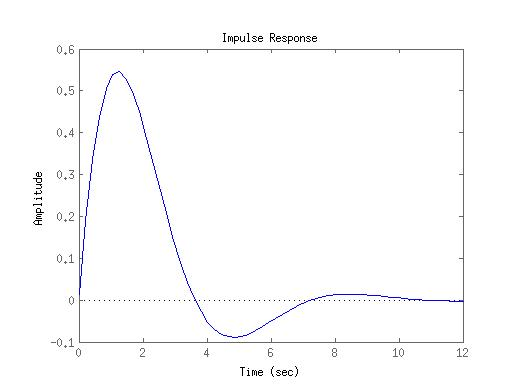
\includegraphics[scale = 0.5]{./images/exerc3-saida-impulso-pro.jpg}
		\caption{resposta com função impulso}
		\label{fig:circuit3-impulso-pro}
\end{figure}
\FloatBarrier


%@@@@@@@@@@@@@@@@@@@@@@@@@@@@@@@@@@@@@@@@@@@@@@@@@@@@@@@@@@@
%@@@@@@@@@@@@@@       Análise         @@@@@@@@@@@@@@@@@@@@@@
%@@@@@@@@@@@@@@@@@@@@@@@@@@@@@@@@@@@@@@@@@@@@@@@@@@@@@@@@@@@
 \newpage
\section{Discussão e Conclusões}
\paragraph{} No experimento 1 vimos como diagramas de blocos com
funções de transferência são facilmente montados e nos fornecem
a resposta a uma determinada entrada rapidamente e de forma
visual. No exercício 2 obtivemos que a saída ao sistema em estudo
tem comportamento exponencial. Em particular a amplitude da grandeza 
de saída tende ao infinito a medida que o tempo cresce, o que é um
comportamento perigoso para a maioria das aplicações. Esse comportamento
não é óbvio ao se olhar apenas o diagrama de bloco, mas se torna evidente
assim que se obtém a simulação. No exercício 3 vimos que ao menos qualitativamente
o impulso pode ser aproximado por um degrau de pequena largura e alta amplitude. 
A resposta obtida por essa aproximação apresenta a mesma forma
mas diverge da resposta ao impulso na escala do gráfico. É possível
que essa resposta melhore se fizermos a largura de pulso diminuir 
mais ainda ao mesmo tempo que elevamos a amplitude do sinal.
%@@@@@@@@@@@@@@@@@@@@@@@@@@@@@@@@@@@@@@@@@@@@@@@@@@@@@@@@@@@
%@@@@@@@@@@@@@@       REFERÊNCIAS     @@@@@@@@@@@@@@@@@@@@@@
%@@@@@@@@@@@@@@@@@@@@@@@@@@@@@@@@@@@@@@@@@@@@@@@@@@@@@@@@@@@
\begin{thebibliography}{9}    
	 \bibitem{ADL-NISE}
  		Nise, N.S.
  		\emph{Engenharia de Sistemas de Controle}
 		 5ª ed.
		LTC, 2009.
	 \bibitem{ADL-OGATA}
  		Ogata, K.
  		\emph{Moder Control Engeeniring}
 		 5ª ed.
		Pearson, 2010.
	 
\end{thebibliography}
\end{document}
